\documentclass[11pt]{article}

\usepackage{thumbpdf, amssymb, amsmath, amsthm, microtype,
	    graphicx, verbatim, listings, color, fancybox}
\usepackage[pdftex]{hyperref}
%\usepackage[margin=1in]{geometry}
\usepackage{cawsty}
\usepackage{fullpage}
\usepackage{pseudocode}
\usepackage{verbatim}
\usepackage{multicol}

\usepackage{fancybox}
\usepackage{tikz}

\newcommand{\tlg}{\text{lg}}
\newcommand{\tln}{\text{ln}}
\newcommand{\tlog}{\text{log}}

\usepackage{algorithm}
%\usepackage{algorithmic}
\usepackage{amsmath}
\usepackage{amsthm}
\usepackage{algpseudocode}
\usepackage{algorithmicx}% http://ctan.org/pkg/algorithmicx
\usepackage{lipsum}% http://ctan.org/pkg/lipsum
\usepackage{xifthen}% http://ctan.org/pkg/xifthen
\usepackage{needspace}% http://ctan.org/pkg/needspace
\usepackage{hyperref}% http://ctan.org/pkg/hyperref

\usepackage{tikz}
\usetikzlibrary{arrows,%
                shapes,positioning}

\tikzstyle{vertex}=[circle,fill=black!25,minimum size=20pt,inner sep=0pt]
\tikzstyle{selected vertex} = [vertex, fill=red!24]
\tikzstyle{edge} = [draw,thick,-]
\tikzstyle{weight} = [font=\small]
\tikzstyle{selected edge} = [draw,line width=5pt,-,red!50]
\tikzstyle{ignored edge} = [draw,line width=5pt,-,black!20]

\allowdisplaybreaks[1]

% ================ ALGORITHM ENVIRONMENT ================
\newcounter{numberedAlg}% Algorithm counter
\newenvironment{numberedAlg}[1][]%
  {% \begin{numberedAlg}[#1]
    \needspace{2\baselineskip}% At least 2\baselineskip required, otherwise break
    \noindent \rule{\linewidth}{1pt} \endgraf% Top rule
    \refstepcounter{numberedAlg}% For correct reference of algorithm
    \centering \textsc{Algorithm}~\thenumberedAlg%
    \ifthenelse{\isempty{#1}}{}{:\ #1}% Typeset name (if provided)
  }{% \end{numberedAlg}
  \noindent \rule{\linewidth}{1pt}% Bottom rule
  }%

%\setlength{\parindent}{0pt}

\linespread{1.2}

\begin{document}
\cawtitle{4005-800 Algorithms}{Homework 7}

\begin{prob}{1 - 34.2-1}
Consider the language GRAPH-ISOMORPHISM = $\{\langle G_1, G_2 \rangle : G_1$ and $G_2$ are isomorphic graphs $\}$. Prove that GRAPH-ISOMORPHISM $\in NP$ by describing a polynomial-time algorithm to verify the language.
\end{prob}
\begin{sol}
By the defintion of graph isomorphism, two graphs $G_1$ and $G_2$ are isomorphic if and only if there exists a bijection $m : V(G_1) \to V(G_2)$ such that any two vertices $v_i$ and $v_j$ of $G_1$ are adjacent in $G_1$ if and only if $m(v_i)$ and $m(v_j)$ are adjacent in $G_2$. In other words, the mapping $m$ is a defines a permutation from $V(G_1) \to V(G_2)$, and we can check to see if this is a valid permutation by checking that for every $v_j \in V(G_2)$, there is exactly one $v_i \in V(G_1)$ such that $m(v_i) = v_j$. We can then check to see that for every edge $(v_i, v_j) \in E(G_1)$, we also have $(m(v_i), m(v_j)) \in E(G_2)$. With these definitions in mind, we can easily devise a polynomial-time algorithm to verify that $m$ is a valid isomorphic mapping as follows:

\begin{numberedAlg}[GRAPH-ISOMORPHISM-VERIFIER]
\label{alg1}
\begin{algorithmic}[1]
	\Function{VerifyGraphIsomorphism}{$m$}
		\ForAll{$v_{j} \in V(G_2)$} 
			\State vCount = 0 \Comment {Count number of times $m(v_i)$ appears in $G_2$}
			\ForAll{$v_i \in V(G_1)$}
				\If{$m(v_i) == v_j$}
					\State vCount = vCount + 1
				\EndIf
			\EndFor
			\If {vCount $\not= 1$} \Comment {$v_i$ should only appear once in $G_2$}
				\State \Return False
			\EndIf
		\EndFor
\\
		\ForAll{$v_i \in V(G_1)$}
			\ForAll{$v_j \in V(G_1)$} \Comment{Check the edge adjacency requirement for the permutation}
				\If{$(v_i, v_j) \in E(G_1)$ and $(m(v_i), m(v_j)) \notin E(G_2)$} 
					\State \Return False 
				\EndIf
				\If{$(m(v_i), m(v_j)) \in E(G_2)$ and $(v_i, v_j) \notin E(G_1)$}
					\State \Return False
				\EndIf
			\EndFor
		\EndFor
\\
		\State \Return True
	\EndFunction
\end{algorithmic}
\end{numberedAlg}

Note that $m$ denotes the bijective mapping (the permutation) from $V(G_1)$ to $V(G_2)$. It is clear that the permutation check runs in $O(V)$ time and the edge check runs in $O(V^2)$ time. Thus, we conclude that this algorithms runs in $O(V^2)$ time and thus verifies the solution (i.e. the permutation mapping $m$) to the GRAPH-ISOMORPHISM problem in polynomial time. 
\end{sol}

\begin{prob}{2 - 34.2-10}
Prove that if $NP \not= co$-$NP$, then $P \not= NP$.
\end{prob}
\begin{sol}
If $NP \not= co$-$NP$, then we know there exists a problem $Q \in NP$ such that $Q \notin co$-$NP$. Therefore, by the definition of set intersection, this means that $Q \notin co$-$NP \cap NP$. Furthermore, it is known that $P \subseteq co$-$NP \cap NP$, which implies that $Q \notin P$. Thus, since $Q \in NP$ and $Q \notin P$ (because $P$ is a subset of $co$-$NP \cap NP$), we conclude that $P \not= NP$. 

%We can also consider the contrapositive of this logical statement...
\end{sol}

\begin{prob}{3 - 34.3-1}
Verify that the circuit in Figure $34.8(b)$ is unsatisfiable.
\end{prob}
\begin{sol}
\begin{center}
	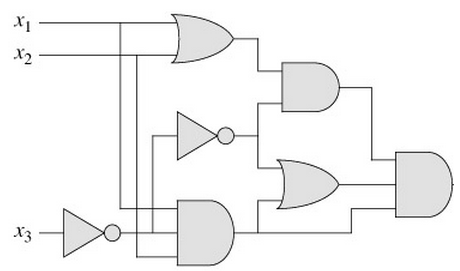
\includegraphics[scale=0.5]{circuit.png} \\
\end{center}

The logical equivalent expression for this circuit is as follows:
\begin{eqnarray*}
((x_1 \lor x_2) \land x_3) \land (x_3 \lor (x_1 \land x_2 \land \lnot x_3)) \land (x_1 \land x_2 \land \lnot x_3)
\end{eqnarray*}

To show that this circuit is unsatisfiable, we simply build a truth table for the boolean expression that considers all logical values for $x_1, x_2,$ and $x_3$, as shown in Table \ref{thetable}:

\begin{table}
\centering
    \begin{tabular}{|l|l|l|l|l|l|}
        \hline
        $x_1, x_2, x_3$ & $x_1 \lor x_2$ & $(x_1 \lor x_2) \land x_3$ & $x_1 \land x_2 \land \lnot x_3$ & $x_3 \lor (x_1 \land x_2 \land \lnot x_3)$ & Final AND Gate \\ \hline
        F,F,F & F & F & F & F & F \\ 
        F,F,T & F & F & F & T & F \\ 
        F,T,F & T & F & F & F & F \\ 
        F,T,T & T & T & F & T & F \\ 
        T,F,F & T & F & F & F & F \\ 
        T,F,T & T & T & F & T & F \\ 
        T,T,F & T & F & T & T & F \\ 
        T,T,T & T & T & F & T & F \\ 
        \hline
    \end{tabular}
	\label{thetable}
	\caption{Truth table for problem \#3, where T = True and F = False.}
\end{table}

Therefore, since there is no possible combination of logical values for $x_1$, $x_2$, and $x_3$ such that the boolean expression is true, we conclude that it is unsatisfiable.

\end{sol}

\begin{prob}{4 - 34.4-5}
Show that the problem of determining the satisfiability of boolean formulas in disjunctive normal form is polynomial-time solvable.
\end{prob}
\begin{sol}
We show that the problem of determining the satisfiability of boolean formulas in disjunctive normal form is polynomial-time solvable by providing a polynomial-time algorithm that performs this task. This algorithm is realized below in Algorithm \ref{alg2}.

\begin{numberedAlg}[DNF-SOLVER]
\label{alg2}
\begin{algorithmic}[1]
	\Function{SolveDNF}{$\psi$}
		\ForAll{Logical clauses $c_i \in \psi$}
			\State $satisfiable = True$
			\State $satList = makeQueue()$
			\ForAll{Literals $l_j \in c_i$}
				\ForAll{Literals $l_k \in satList$}
					\If{$l_k == \lnot l_j$}
						\State $satisfiable$ = False \Comment{Found the negation of $l_j$ in the queue}
					\EndIf
				\EndFor
				\State $PUSH(satList, l_j)$ \Comment{Push this literal into the queue}
			\EndFor
			\If{$satisfiable == True$} 
				\State \Return $True$ \Comment{Found one clause that can be satisfied}
			\EndIf
		\EndFor
		\State \Return $False$
	\EndFunction
\end{algorithmic}
\end{numberedAlg}

Since DNF statements are composed of disjunctions (ORs) of conjunction clauses (ANDs), it is enough to check and see if only one conjunction clause can be satisfied. Therefore, this procedure simply traverses over every clause and checks to see if there is a literal and its negation in that clause, which indicates that the clause can never be true. If this is not the case, then the clause must be satisfiable, and thus the expression is satisfiable. 

The time complexity of this algorithm is $O(mn^2)$, where $m$ is the number of clauses in $\psi$ and $n$ is the number of literals in the boolean expression. The reason for this is that for every clause we traverse over every literal in the clause, and for each element we perform a linear search with $satList$ that can be equal to the number of literals in the clause. Therefore, since the linear search runs in $O(n)$ time, the number of literals in a clause is $O(n)$, and the number of clauses in $\psi$ is $O(m)$, and each of these operations are nested, the resulting time complexity is $O(mn^2)$.
\end{sol}

\begin{prob}{5 - 34.5-5}
The \textbf{set-partition problem} takes as input a set $S$ of numbers. The question is whether the numbers can be partitioned into two sets $A$ and $A' = S - A$ such that $\sum_{x \in A}x = \sum_{x \in A'} x$. Show that the set-partition problem is $NP$-complete.
\end{prob}
\begin{sol}
In order to show that the set-partition problem $Q$ is $NP$-complete, we show that it can be reduced from the subset-sum problem $Q'$, which is also $NP$-complete. That is, we prove $Q' \leq_p Q$ as follows:

%x \in L_1 iff f(x) \in L_2 -> state this requirement for reducibility (taken from textbook)

\begin{itemize}
	\item First, we must show that $Q \in NP$. To do this, we show that a certicate of $Q$ can be verified in polynomial time. Suppse such a certificate of $Q$ contains two partite subsets $A$ and $A'$ of an input set $S$ of numbers. We can easily compute the sum of all elements in both $A$ and $A'$ in $O(n)$ time and then compare if these sums are equivalent in constant time. Thus, the certficate of $Q$ can be verified in polynomial time ($O(n)$), and so we conclude that $Q \in NP$. 

	\item Now we need to show that $Q' \leq_p Q$. To do so, we define a construction technique that translates instances of $Q'$ to instances of $Q$ as follows. Let $S$ be a set of numbers that contains a subset $S' \subseteq S$ that sum to the integer target $t$. We denote $s = \sum_{x \in S}x$, and with this we construct a new set $S^*$ as $S \cup \{s - 2t\}$. The reasoning behind this construction is that the set $S'' = S - S'$ has a sum of $s - t$, and so if we add the number $s - 2t$ to $S$ we are guaranteed that by including this number in $S'$ we are left with a total sum of $t + s - 2t = s - t$. Thus, there will be two partite sets that sum to exactly $s - t$.

	\item Suppose we have a satisfiable instance of $Q'$ that consists of a set of numbers $S$ and a subset of $S' \subseteq S$ that sums to an integer target $t$. Applying the construction technique described above, we are left with a new set $S^*$, where we have the following:
\begin{eqnarray*}
\sum_{x \in S^*}x &=& (s + (s - 2t))\\
& = & (t + (s - t) + (s - 2t) \text{ (Split up the subsets in $S$ that sum to $s$ and $s - t$}\\
& = & (s - t) + (s - 2t + t) \text{ (Include $s - 2t$ in $S'$)}\\
& = & 2(s - t)
\end{eqnarray*}
Therefore, we know that there are exactly two partite sets in $S$ that sum to exactly $s - t$, and thus $S$ is an instance of $Q'$ that can be used to construct $S^*$, which also satisfies $Q$.

	\item Now, suppose we have a satisfiable instance of $Q$ that contains two partitite sets $A$ and $A'$, where $\sum_{x \in A}x = \sum_{x \in A'}x = (s - t)$. By our construction technique, we know that one of these partite sets contains the number $m = s - 2t$, and if we remove that number from the corresponding set we are left with $s - t - (s - 2t) = t$. Therefore, since $S^* - \{m\} = S$ and there is a subset in $S$ that now sums to $t$, we conclude that this instance of $Q$ also satisfies $Q'$.

%http://web.njit.edu/~marvin/cs341/hw/hwsoln13.pdf

%$\sum_{x \in S^*}x = 2(s - t) = 2s - 2t = s + (s - 2t)$. Therefore, we know that there is subset of $S' \subseteq S^*$ such that $\sum_{x \in S'}x = s - 2t$. Now, if we consider the set $S = S^* - S'$, then we know that $\sum_{x \in S}x = s + (s - 2t) - (s - 2t) = s$. 

	\item Finally, we show that the construction of $S^*$ can be done in polynomial time from an instance of $Q'$ simply by computing the sum $s - 2t$, which is done in $O(n)$ time by traversing over all of the elements in $S$, and then including it in the set $S$ in constant time. 
\end{itemize}

Thus, since we defined a polynomial time construction that transforms satisfiable instances of $Q'$ to $Q$, and such instances satisfy both $Q$ and $Q'$, we conclude that $Q' \leq_p Q$. Now, since $Q'$ is $NP$-complete, we can also conclude that $Q$ (the set-partition problem) is $NP$-complete.
\end{sol}

\begin{prob}{6-a}
Write pseudo-code for a recursive solution to the variation on the 0-1 knapsack problem that computes the
maximum value that can be placed in the knapsack.
\end{prob}
\begin{sol}
\begin{numberedAlg}[RECURSIVE 0-1 KNAPSACK]
\label{alg2}
\begin{algorithmic}[1]
	\Function{RecursiveKnapsack}{$n, v, w, W$}
		\If{$n == 0$} \Comment{There are no items to contribute weight or value}
			\State \Return $0$ 
		\ElsIf{$W < w[n]$} \Comment{This item is too heavy, so don't include it}
			\State \Return $RecursiveKnapsack(n-1, v, w, W)$
		\Else 
			\State \Return max($v[n]+RecursiveKnapsack(n-1, v, w, W-w[n])$, \\ $RecursiveKnapsack(n-1,v,w,W)$)
		\EndIf
	\EndFunction
\end{algorithmic}
\end{numberedAlg}
\end{sol}

\begin{prob}{6-b}
Give a dynamic programming solution to the 0-1 knapsack problem that is based on the previous problem;
this algorithm should return the items to be taken. Implement this algorithm and call it $knapsack$.
\end{prob}
\begin{sol}
The source code for the dynamic programming solution to the 0-1 knapsack problem is given below.

\begin{lstlisting}
def knapsack(n, values, weights, capacity):
	table = list() 
	for i in range(0, n):
		rowList = list()
		for j in range(0, capacity + 1):
			rowList.append(0)
		table.append(rowList)		
	for i in range(0, n):
		for w in range(0, capacity + 1):
			if (weights[i] > w):
				table[i][w] = table[i - 1][w]
			else:
				vIn = values[i] + table[i - 1][w - weights[i]]
				vOut = table[i - 1][w]
				table[i][w] = max(vIn, vOut)
	return getItemIndices(table, n, weights, capacity)

def getItemIndices(values, n, w, capacity):
	i = len(values) - 1
	weight = capacity
	indices = []	
	for i in range(0, n):
		indices.append(0)
	while i >= 0 and weight >= 0:
		if ((i == 0 and values[i][weight] > 0) or 
			(values[i][weight] != values[i - 1][weight])):
			indices[i] = 1
			weight = weight - w[i]
		i = i - 1
	return indices
\end{lstlisting}
\end{sol}

\begin{prob}{6-c}
What is the time complexity of your dynamic programming based algorithm?
\end{prob}
\begin{sol}
The time complexity of this dynamic programming based algorithm depends on the computation of the $value$ table and identifying the items that were added to the knapsack. Since these procedures are run back-to-back, we consider their time complexity separately in order to determine the time complexity of the entire algorithm.

The time complexity of the value computation depends on the initialization procedure in which the table is constructed and then the nested loops that perform the bottom-up computation. The initialization procedure generates a table that has dimensions $n \times W$, so it runs in $O(nW)$ time. Similarly, the table computation procedure performs a constant time table lookup (or returns a $0$ in the base case) when traversing across every possible knapsack capacity for every item, so we can conclude that this procedure runs in $O(nW)$ time as well.

Analyzing the time complexity of the item identification procedure indicates that it runs in $O(n)$ time, because at every iteration through the main loop the item counter is decreased by $1$ until we consider all items in the knapsack. Hence, the linear time complexity of $O(n)$.

Now, putting these two results together, the dynamic programming based algorithm that solves the 0-1 knapsack problem has a time complexity of $O(nW) + O(nW) + O(n)$, which can be reduced to $O(nW)$. 
\end{sol}

\begin{prob}{6-d}
The knapsack decision problem is $NP$-complete. Does your analysis above prove that $P = NP$? Explain.
\end{prob}
\begin{sol}
%TODO: http://en.wikipedia.org/wiki/Knapsack_problem
%http://stackoverflow.com/questions/3907545/how-to-understand-the-knapsack-problem-is-np-complete
No, this analysis does not prove that $P = NP$, because the $O(nW)$ time complexity depends on the value of $W$, not the size of $W$. Time complexity measurements consider the size of the input of an algorithm (i.e. the number of bits if the input is a numeric value), and since $W = 2^{\tlg W}$, where $\tlg W$ is the number of bits in $W$, we can see that the resulting time complexity is thus $O(n2^{\tlg W})$ in terms of the size of $W$. This means that this dynamic programming solution is a pseudo-polynomial time algorithm in that it is polynomial with respect to the value of the input, but exponential with respect to the size of the input, and thus is not polynomial in the traditional sense. Therefore, we can see that this does \emph{not} prove that $P = NP$.

\begin{comment}
time complexity comes from the number of bits that are used to represent $W$, not the value of $W$. As the weight capacity of the knapsack increases the number of individual items that can be stored in $W$ increases by individual items as well, and if we treat $W$ as a binary number then we also say that the number of bits used to store $W$ increases by 1. However, by increasing the number of bits in $W$ in a linear manner, we increase the value of $W$ exponentially. Thus, we can conclude that this dynamic programming problem runs in psuedo-polynomial time, which means that it ultimately runs in exponential time complexity. Therefore, this solution is still in $NP$, so we cannot conclude that $P = NP$.
\end{comment}
\end{sol}

\end{document}
